\section{Benutzeroberfläche}
\vspace{1cm}

Die Benutzeroberfläche des Systems ist vor allem auf Bedienbarkeit ausgelegt. Sie wird übersichtlich gestaltet und erfordert keine Einstellungen durch die Nutzer. Wir orientieren uns beim Design der Bedienelemente auf den Ergebnissen von Benedikt Bieberle, Niclas Deppisch und Robert Schwartz: "`Prototypische Entwicklung eines Self-Service-Terminals für Wartebereiche von Krankenkassenfilianen"', Medienprojekt TU Ilmenau, Mai 2020, dass sich mit der Aktzeptanz und Bedienbarkeit einer Benutzeroberfläche für eben jenen Anwendungsfall beschäftigt, für den wir entwickeln.

\vspace{1,5cm}
\subsection{Bildschirmlayout}
\vspace{1cm}
Das Bildschirmlayout ist für das 9 Zoll IPad mit Toucheingabe ausgelegt. Um einfache Bedienbarkeit zu gewährleisten, werden wenige, große Schaltflächen mit gut lesbarer Schrift verwendet. Wir lehnen uns beim Design an das Ergebnis eines Medienprojekts an der TU Ilmenau an, das zwei verschiedene Designs miteinander verglichen hat. Wir haben uns für das visuell einfachere Design entschieden, da es sich gezeigt hat, dass Kunden diese Oberfläche schneller bedienen können.\par
\newpage
\noindent Das Layout ist für den Hochkant-Betrieb designt. Zusätzlich zu im Medienprojekt verwendeten Darstellungen, fügen wir eine Schaltfläche ein, die direkt zum Startbildschirm führt.\par
\vspace{1cm}
\textbf{Layout:}

\begin{figure}[htp]
    \centering
    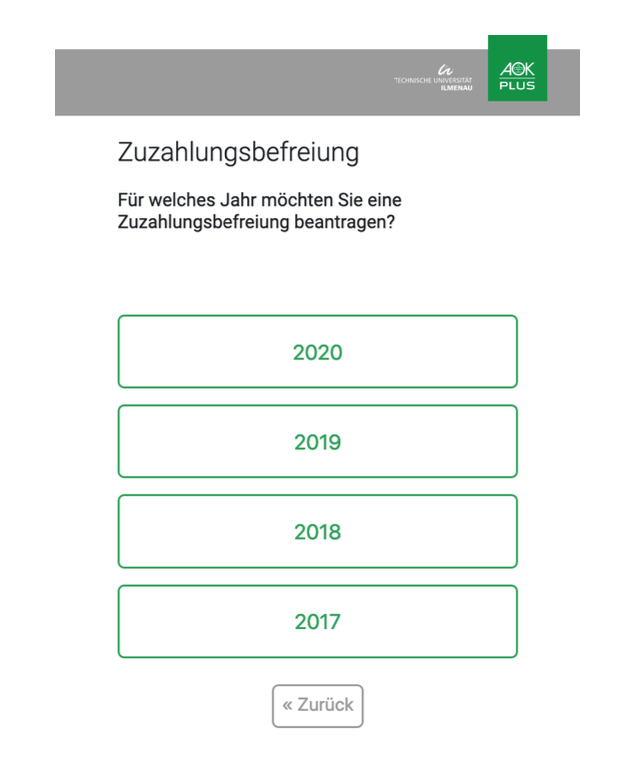
\includegraphics[width=10cm , height=12cm]{Bilder/Interface.png}
    \caption{Benedikt Bieberle, Niclas Deppisch und Robert Schwartz, "`Prototypische Entwicklung eines Self-Service-Terminals für Wartebereiche von Krankenkassenfilianen"', Medienprojekt TU Ilmenau, Mai 2020}
    \label{fig:Interface}
\end{figure}
